\chapter{Un \textit{wearable device} pour la reconnaissance des sols}
\label{chap:4}

\section{Introduction}

Au cours des dernières années, les \textit{wearable devices} ont gagné en popularité, poussée par les grands fabricants de matériel tels que \textit{Garmin}, \textit{Apple}, \textit{Samsung} ou encore \textit{Fitbit}. En effet, selon le rapport réalisé par \cite{Nielsen2014}, 70\% des consommateurs interrogés connaissent cette technologie et 15\% d'entre eux se servent d'un \textit{wearable device} dans leur vie de tous les jours en plus de leur téléphone intelligent. Ces dispositifs ont permis l'exploitation de nouveaux types de capteurs, en comparaison de ceux qui étaient déjà présents dans les téléphones (\textit{p. ex.} les capteurs cardiaques) et ils ont permis d'accélérer l'adoption de technologies comme le \acs{BLE} \citep{Taplett}. En ce sens, et puisqu'ils représentent un moyen pratique et portable pour enregistrer des données physiologiques,  les \textit{wearable devices} ont été rapidement et massivement adoptés, principalement pour assurer le suivi des activités sportives \citep{NPDGroup2015}. Il est donc devenu possible, pour leurs utilisateurs, de récolter une quantité considérable de données dans le but de produire des analyses statistiques et ainsi surveiller les évolutions dans la réalisation d'activités quotidiennes, qu'elles soient sportives ou non. Néanmoins, avec les avancements en matière d'apprentissage machine, il est possible d'affirmer que les applications développées spécifiquement pour les \textit{wearables devices} peuvent être améliorées pour devenir plus ubiquitaires.

L'objectif de ce chapitre est donc d'introduire un nouveau cas d'utilisation d'un wearable device ou la réponse à la question suivante : \textit{« Est-il possible de reconnaître les types de sols à l'aide de données inertielles produites par la démarche humaine avec un wearable device\textemdash quel que soit l'endroit où il se trouve et par qui il est porté ? »} est le principal sujet discuté dans deux publications respectivement présentées aux conférences \textit{IEEE 14th International Conference on Ubiquitous Intelligence and Computing (UIC)} qui s'est déroulée en août 2017 à San Francisco aux États-Unis \citep{Thullier2017a} et \textit{IEEE 15th International Conference on Ubiquitous Intelligence and Computing (UIC)} qui s'est déroulée en octobre 2018 à Guangzhou en Chine \citep{Thullier2018}.

Pour se faire, ce chapitre commence par présenter un état de l'art des recherches menées au sujet de la reconnaissance des sols par le biais de données inertielles. Ensuite, après avoir présenté la solution proposée ainsi que les expérimentations réalisées, ce chapitre va analyser et discuter les résultats obtenus. Finalement, la dernière partie dresse une conclusion de ce premier travail.

\section{État de l'art}

L'idée de reconnaître des types de sols par le biais de données produites par une centrale inertielle vient du domaine de la robotique. En effet, \cite{Vail2004} ont tout d'abord expérimenté la détection de surface grâce à des données inertielles produites par un robot quadrupède. Pour réaliser l'apprentissage, les auteurs ont opté pour un algorithme dont le modèle est un arbre de décision ($C4.5$), car ils estiment qu'il s'agit d'un algorithme suffisamment rapide et facile à représenter et à implémenter. Pour quantifier la précision de leur modèle d'apprentissage, \citeauthor{Vail2004} ont utilisé la technique de la validation croisée en 10-plis \citep{Kohavi1995}, ce qui leur a permis d'obtenir un taux de reconnaissance global de 84.9\% (ciment: 91\%; tapis: 81.2\%; champs: 81.2\%). Par la suite, \cite{Kertesz2016} ont également présenté une méthode permettant de reconnaître des sols avec un accéléromètre embarqué sur un robot quadrupède. Ceux-ci ont obtenu un taux de confiance de 96.2\% en utilisant l'algorithme \textit{Random Forest} et en évaluant la précision de l'apprentissage avec la même technique que celle utilisé par \citeauthor{Vail2004}. La différence majeure entre les deux travaux réside principalement dans le fait que les premiers ont utilisé des caractéristiques temporelles du signal inertiel (variance et correlation) pour concevoir leur modèle d'apprentissage, tandis que les seconds ont utilisé des caractéristiques fréquentielles grâce à une \acs{FFT}.

Par ailleurs, \cite{Bibuli2007} ont proposé une méthode de reconnaissance des sols pour un robot à quatre roues équipé de plusieurs types de capteurs, dont une centrale inertielle. Pour ce faire, ils ont tout d'abord calculé les composantes fréquentielles du signal inertiel \textit{via} l'algorithme de la transformée de fourrier discrète (\acl{DFT} ou \acs{DFT}), pour chacun des axes du capteur. Chaque ensemble a ensuite été entrainé distinctement par son propre réseau de neurones artificiels (\acs{ANN}). Par conséquent, les meilleurs résultats ont été obtenus avec les données de l'axe $x$ du gyroscope, soit respectivement 90\%, 71.2\%, 70\%, 98.8\% et 83.5\% pour les sols en graviers, gazon, sable, pavés et terre. 

Enfin, \cite{Weiss2007} ont proposé une comparaison de plusieurs méthodes pour réaliser une reconnaissance de sols avec un robot à quatre roues doté d'un capteur inertiel. Plus précisément, ils ont comparé l'algorithme \acs{SVM} avec d'autres types d'algorithmes d'apprentissage où les données fournies en entrées sont des caractéristiques fréquentielles du signal inertiel correspondant à différentes vitesses du robot (0.2, 0.4 et 0.6 $m/s$) et pour six sols distincts (sol intérieur, asphalte, gravier, gazon, pavés, sol argileux). Avec l'obtention de 77\% de taux de confiance, leur étude a montré de meilleurs résultats avec l'algorithme \acs{SVM} qu'avec les autres algorithmes utilisés comme un réseau de neurones probabiliste (\acl{PNN} ou \acs{PNN}), l'algorithme des $k$ plus proches voisins, l'algorithme bayésien naïf ou encore $C4.5$.

Bien que cette littérature soit, d'une certaine manière, pertinente pour comprendre comment reconnaître différents types de sols, il est possible que ces méthodes ne soient pas parfaitement adaptées pour effectuer une reconnaissance appropriée dans le contexte de la démarche humaine. Au mieux de notre connaissance, il apparait que peu de recherches ont été proposées pour exploiter une telle reconnaissance avec l'humain. Pourtant, de nombreux cas d'utilisation à la reconnaissance des sols dans ce contexte nous paraissent exploitables. Le premier exemple concerne le domaine sportif où il serait possible de subdiviser un tracé \acs{GPS} en de plus petits tracés déterminés par rapport à la composition du sol et ainsi fournir des détails supplémentaires sur un sentier de randonnée ou de course. Dans un second temps, une telle technologie pourrait être utile au domaine de la santé et plus particulièrement de celui de l'assistance. En effet, avec la connaissance du type de sol, il serait possible de proposer des techniques de prévention des chutes plus efficaces puisque celles-ci sont plus susceptibles de survenir lorsque les personnes évoluent sur certains types de sols (\textit{p. ex.} le carrelage humide d'une salle de bain).

De ce fait, \cite{Otis2016} ont récemment proposé une méthode basée sur la reconnaissance des types de sols pour réduire les risques de chutes qui demeurent particulièrement importants chez les personnes en perte d'autonomie ou plus simplement, les personnes âgées. Pour ce faire, une chaussure embarquant un accéléromètre a été fabriquée. Ensuite, un algorithme de \textit{clustering} a été utilisé pour segmenter les caractéristiques fréquentielles discriminantes obtenues par le biais de la \acs{FFT} sur le signal accéléromètrique lorsque celui-ci a été enregistré sur les sols suivants : gravier, ciment sable, neige et glace. En ce qui concerne les résultats obtenus, les auteurs mentionnent un taux d’identification erronée compris entre 1\% et 5\% lors des essais en laboratoire, alors qu’ils ont observé une augmentation du taux d'erreur à 20\% en conditions réelles.

\section{Solution proposée}

\subsection{Le \textit{wearable device}}

Selon la littérature existante, l'utilisation de centrales inertielles pour réaliser la reconnaissance de sols s'est montré une technique aussi bien fonctionnelle avec des robots qu'avec les individus. De ce fait, la contribution présentée dans ce chapitre s'est, dans un premier temps, axée sur la conception d'un \textit{wearable device} pour y parvenir. L'idée générale est de piloter, par l'intermédiaire d'un téléphone connecté en \acs{BLE}, le dispositif afin d'enregistrer un volume important de données pendant une marche. Lors de la conception, le choix s'est porté sur le système sur puce (\acl{SOC} ou \acs{SOC}) \textit{Arduino 101} qui embarque le module \textit{Intel Curie}. Celui est également accompagné d'un \textit{shield} de prototypage sur lequel est embarqué un lecteur de carte mémoire, tel qu'illustré en figure \ref{fig:device}. Ce choix a été motivé par la composition même du module \textit{Intel Curie}. En effet, ce dernier intègre d'usine un module de communication \acs{BLE}, un \acs{IMU} 6 axes (6-\acl{DOF} ou 6-\acs{DOF}) ainsi qu'une quantité suffisante d'Entrées/Sorties (\acl{IO} ou \acs{IO}) pour connecter des composants supplémentaires comme un autre IMU comportant plus d'axes. De plus, les autres avantages au choix de ce matériel demeurent la simplicité et la fiabilité de l'\textit{Arduino 101}, mais également la quantité de ressources disponibles pour cette plateforme. Finalement, la présence d'un lecteur de carte mémoire sur le \textit{shield} de prototypage constitue un moyen simple et efficace pour faire face à la quantité de données inertielles qui doivent être stockées.

Dans une première version, la reconnaissance des types de sols a été réalisée par l'intermédiaire de l'IMU 6-\acs{DOF} directement embarqué sur le \acs{SOC} \textit{Arduino}. Néanmoins, puisque la précision de celui-ci était inconnue avant les premières expérimentations et qu'il manquait les trois axes supplémentaires du magnétomètre, une seconde version du \textit{wearable device} a été proposée. Pour cette dernière, un nouvel IMU 9-\acs{DOF}, le \textit{LSM9DS1}, a été interfacé directement sur le \textit{shield} de prototypage.

\begin{figure}[H]
	\centering
	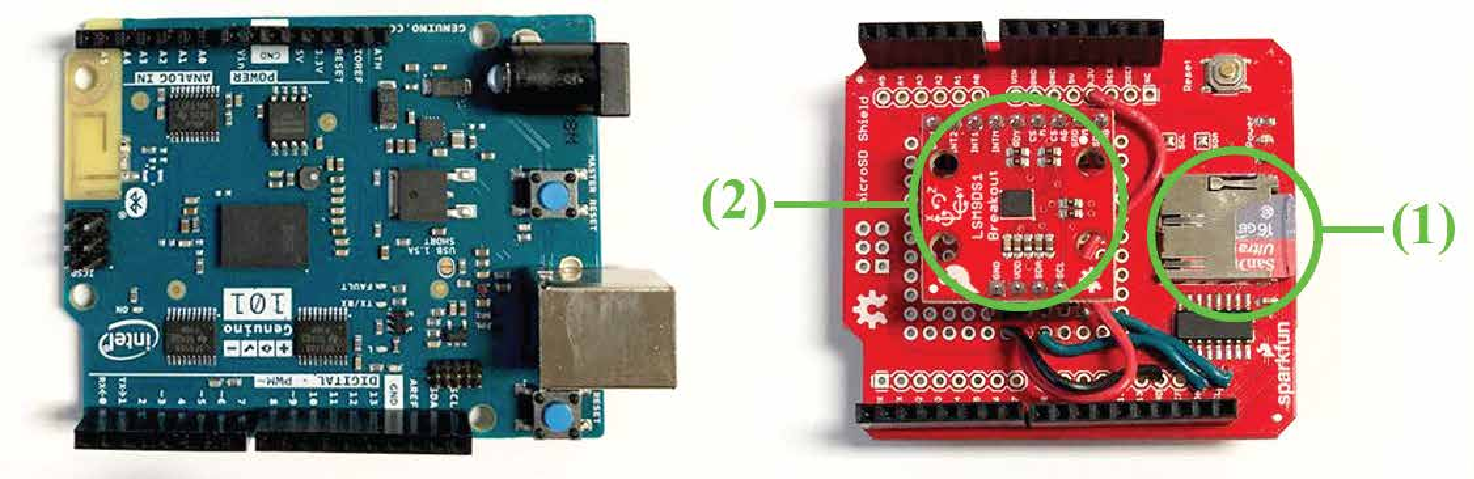
\includegraphics[width=.8\linewidth]{device.pdf}
        \caption{\acs{SOC} Arduino 101 et son \textit{shield} de prototypage incluant une carte mémoire (1) ainsi que la centrale inertielle \textit{LSM9DS1} (2) présente sur la version 2 du dispositif.}
	\label{fig:device}
\end{figure}

\subsection{Le \textit{firmware}}

Pour assurer le bon fonctionner du matériel qui compose le \textit{wearable device} le développement d'un \textit{firmware} \citep{Thullier2019} était requis. Le fonctionnement de celui-ci s'articule autour de trois composants logiciels principaux qui sont illustrés en figure \ref{fig:soil_types_firmware}.

\begin{figure}[H]
	\centering
	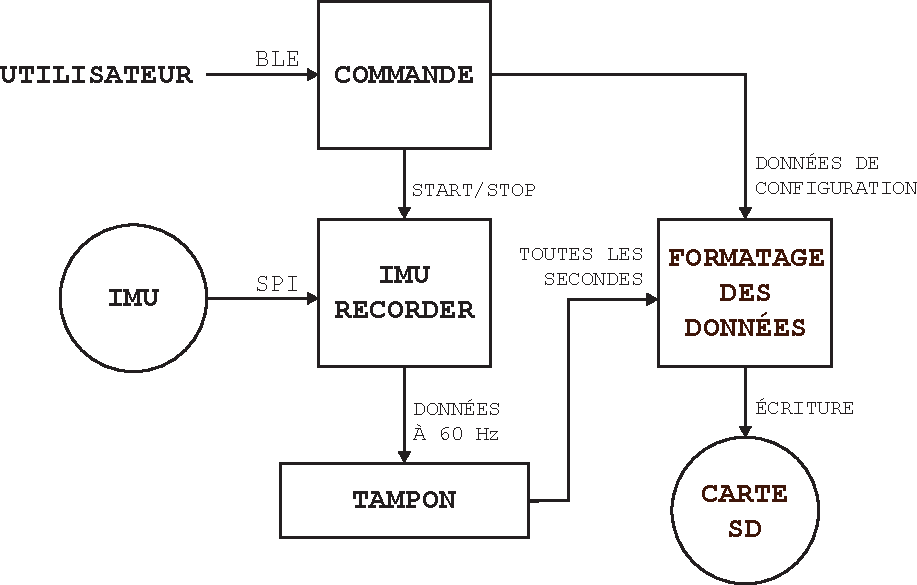
\includegraphics[width=12cm]{soil_types_firmware.pdf}
        \caption{Représentation graphique de l'implémentation du \textit{firmware} embarqué sur le \textit{wearable device}.}
	\label{fig:soil_types_firmware}
\end{figure}

Le premier est le module de commande. Il est en charge des communications entre le téléphone et le dispositif par l'intermédiaire du module radio \acs{BLE}. Ainsi, un téléphone ou n'importe quel autre dispositif compatible avec la technologie \acs{BLE} peut être utilisé pour étiqueter les ensembles de données enregistrés avec les paramètres requis (le type de sol, l'identifiant du participant et l'emplacement du dispositif).

Le second module principal est l'\textit{\acs{IMU} Recorder}. En fonction de la version du dispositif, il a pour rôle de stocker dans une mémoire tampon les valeurs de l'\acs{IMU} qui transitent soit par un bus de données \ac{SPI} dans sa première version, soit \textit{via} un bus de données \ac{I2C}, à une fréquence stabilisée à $60\: Hz$.

Le contenu de la mémoire tampon est ensuite envoyé au module de formatage des données toutes les secondes. Finalement, ce composant récupère l'ensemble des données de configuration du module de commande et s'occupe d'écrire les nouvelles données dans un fichier \ac{CSV} qui est stocké sur la carte mémoire. Dans la seconde version du \textit{wearable device}, le module de formatage des données s'occupe également de calculer les angles d'Euler grâce aux trois axes du \textit{LSM9DS1}.

\subsection{Le processus d'apprentissage pour la reconnaissance des types de sols}

Après que les données aient été enregistrées sur la carte mémoire, le processus d'apprentissage pour la reconnaissance des types de sol est réalisée. Celui-ci débute par l'extraction des caractéristiques. En ce sens, cette solution propose d'utiliser les caractéristiques temporelles et fréquentielles les plus employées dans le domaine de la reconnaissance d'activités tel que discuté à la section \ref{sec:prel_steps} et qui sont rappelées par le tableau \ref{tab:features}. la première opération consiste en une simple moyenne non pondérée sur chacun des axes des capteurs de l'\acs{IMU} (gyroscope, accéléromètre, magnétomètre si 9-\acs{DOF}). Ensuite, la moyenne de chacune de ces caractéristiques est calculée pour chaque capteur de la centrale inertielle. De la même manière, cette procédure a été appliquée à plusieurs autres calculs statistiques : l'écart type, l'asymétrie (équation \ref{eq:asymetrie}), le kurtosis (équation \ref{eq:kurtosis}), le \textit{Zero Crossing Rate} et la correlation entre toutes les combinaisons possibles d'axes par capteurs de l'\acs{IMU} (équation \ref{eq:correlation}). Dans un second temps, une tranfromation du domaine temporel vers le domaine fréquentiel a été nécéssaire pour obtenir les caractéristiques suivantes : la composante continue, l'énergie spectrale (équation \ref{eq:energy_spec}) et l'entropie  (équation \ref{eq:entropy}). Cette transformation a été réalisée en utilisant l'algorithme de la tranformation de Fourier rapide (\acs{FFT}). Ainsi, en fonction de la centrale intertielle exploitée (6-\acs{DOF} ou 9-\acs{DOF}), ce sont soit 70 soit 105 caractéristiques qui sont calculées sur chaque fênetre non-chevauchante fixe de 60 secondes et pour chacun des signaux bruts.

\begin{table}[H]
	\caption{Récapitulatif de toutes les caractéristiques utilisées par la solution proposée en fonction du nombre d'axes offerts par la centrale inertielle.}
	\label{tab:features}
	\resizebox{\textwidth}{!}{%
	\begin{tabular}{|r|c|c||c|c|c|}
	\hline
	\multicolumn{3}{|c||}{\textbf{Domaine Temporel}} & \multicolumn{3}{c|}{\textbf{Domaine Fréquentiel}} \\ \hline
	\multicolumn{1}{|c|}{\multirow{2}{*}{\textit{\textbf{Caractéristique}}}} & \multicolumn{2}{c||}{\textit{\textbf{\begin{tabular}[c]{@{}c@{}}Nb. Total de\\[-15pt] Caractéristiques\end{tabular}}}} & \multirow{2}{*}{\textit{\textbf{Caractéristique}}} & \multicolumn{2}{c|}{\textit{\textbf{\begin{tabular}[c]{@{}c@{}}Nb. Total de\\[-15pt] Caractéristiques\end{tabular}}}} \\ \cline{2-3} \cline{5-6}
	\multicolumn{1}{|c|}{} & \textit{\begin{tabular}[c]{@{}c@{}}IMU \\[-15pt] 6 axes\end{tabular}} & \textit{\begin{tabular}[c]{@{}c@{}}IMU \\[-15pt] 9 axes\end{tabular}} &  & \begin{tabular}[c]{@{}c@{}}IMU \\[-15pt] 6 axes\end{tabular} & \begin{tabular}[c]{@{}c@{}}IMU \\[-15pt] 9 axes\end{tabular} \\ \hline
	Moyenne pour chaque axe & 6 & 9 & \multicolumn{1}{r|}{Composante continue pour chaque axe} & 6 & 9 \\ \hline
	Moyenne de tous les axes & 2 & 3 & \multicolumn{1}{r|}{\begin{tabular}[c]{@{}r@{}}Énergie spectrale pour chaque axe\\[-15pt] (équation \ref{eq:energy_spec})\end{tabular}} & 6 & 9 \\ \hline
	Écart type pour chaque axe & 6 & 9 & \multicolumn{1}{r|}{\begin{tabular}[c]{@{}r@{}}Entropie pour chaque axe\\[-15pt] (équation \ref{eq:entropy})\end{tabular}} & 6 & 9 \\ \hline
	Écart type pour tous les axes & 2 & 3 & - & - & - \\ \hline
	\begin{tabular}[c]{@{}r@{}}Asymétrie pour chaque axe\\[-15pt] (équation \ref{eq:asymetrie})\end{tabular} & 6 & 9 & - & - & - \\ \hline
	Asymétrie pour tous les axes & 2 & 3 & - & - & - \\ \hline
	\begin{tabular}[c]{@{}r@{}}Kurtosis pour chaque axe\\[-15pt] (équation \ref{eq:kurtosis})\end{tabular} & 6 & 9 & - & - & - \\ \hline
	Kurtosis pour tous les axes & 2 & 3 & - & - & - \\ \hline
	\begin{tabular}[c]{@{}r@{}}Corrélation entre toutes les combinaisons \\[-15pt] possibles d'axes incluant le total des axes \\[-15pt] (équation \ref{eq:correlation})\end{tabular} & 12 & 18 & - & - & - \\ \hline
	Zero Crossing Rate pour chaque axe & 6 & 9 & - & - & - \\ \hline
	Zero Crossing Rate pour tous les axes & 2 & 3 & - & - & - \\ \hline
	\textit{\textbf{Sous-total}} & \textit{\textbf{52}} & \textit{\textbf{78}} & \multicolumn{1}{r|}{\textit{\textbf{Sous-total}}} & \textit{\textbf{18}} & \textit{\textbf{27}} \\ \hline\hline
	\multirow{2}{*}{\textbf{Total}} & \multicolumn{1}{r|}{\textit{\textbf{\begin{tabular}[c]{@{}r@{}}IMU\\[-15pt] 6 axes\end{tabular}}}} & \multicolumn{4}{c|}{\textbf{70}} \\ \cline{2-6}
	 & \multicolumn{1}{r|}{\textbf{\begin{tabular}[c]{@{}r@{}}IMU\\[-15pt] 9 axes\end{tabular}}} & \multicolumn{4}{c|}{\textbf{105}} \\ \hline
	\end{tabular}
	}
\end{table}

\subsubsection{Apprentissage}

\begin{figure}[H]
	\centering
	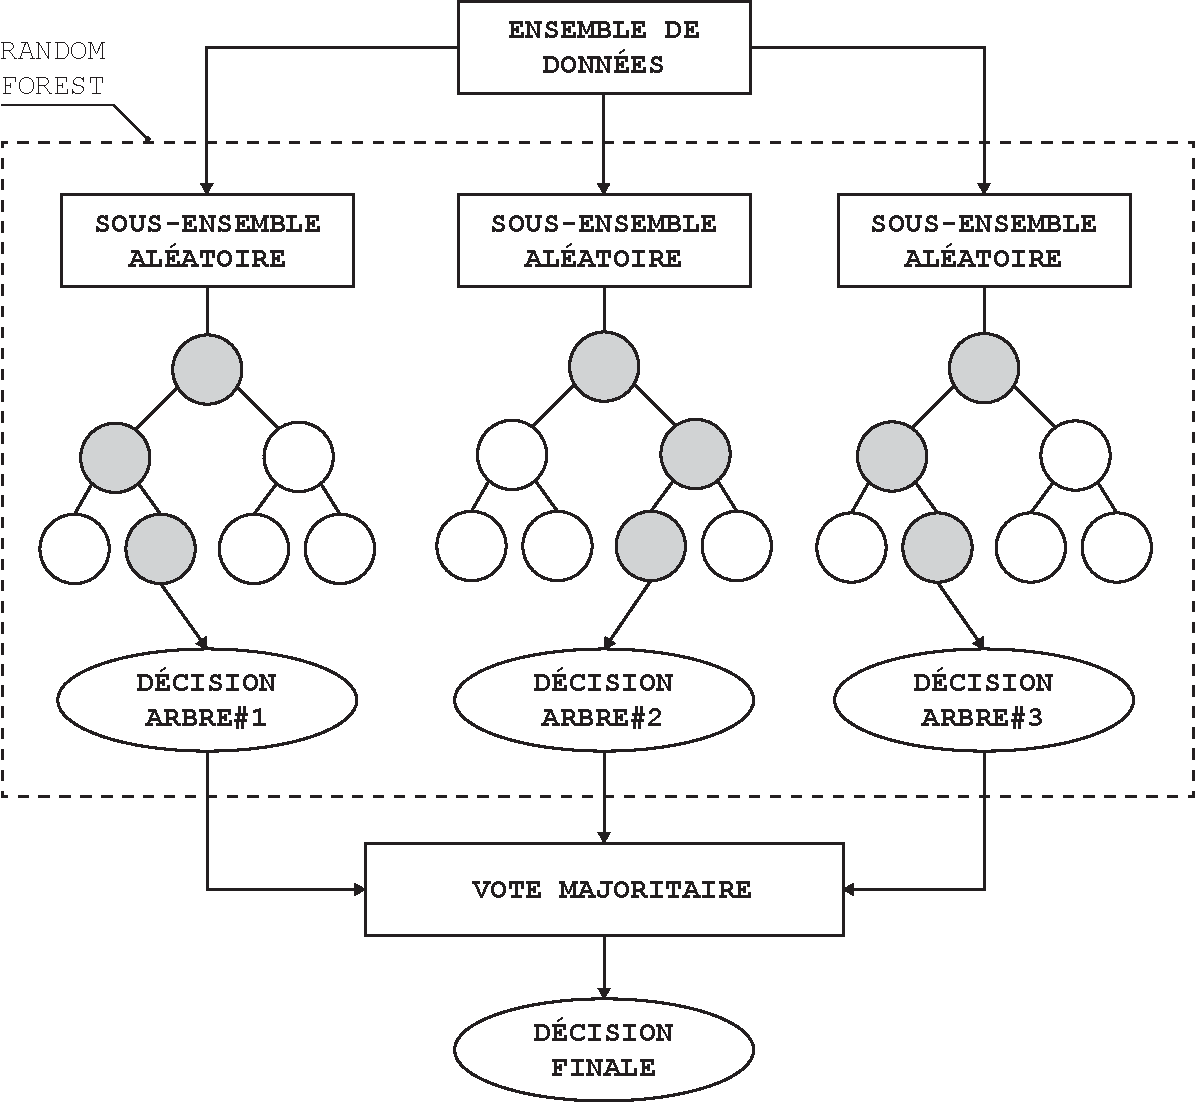
\includegraphics[width=12cm]{algo_random_forest.pdf}
        \caption{Exemple de l'algorithme \textit{Random Forest} utilisant $B=3$ arbres.}
	\label{fig:algo_random_forest}
\end{figure}

\begin{figure}[H]
	\centering
	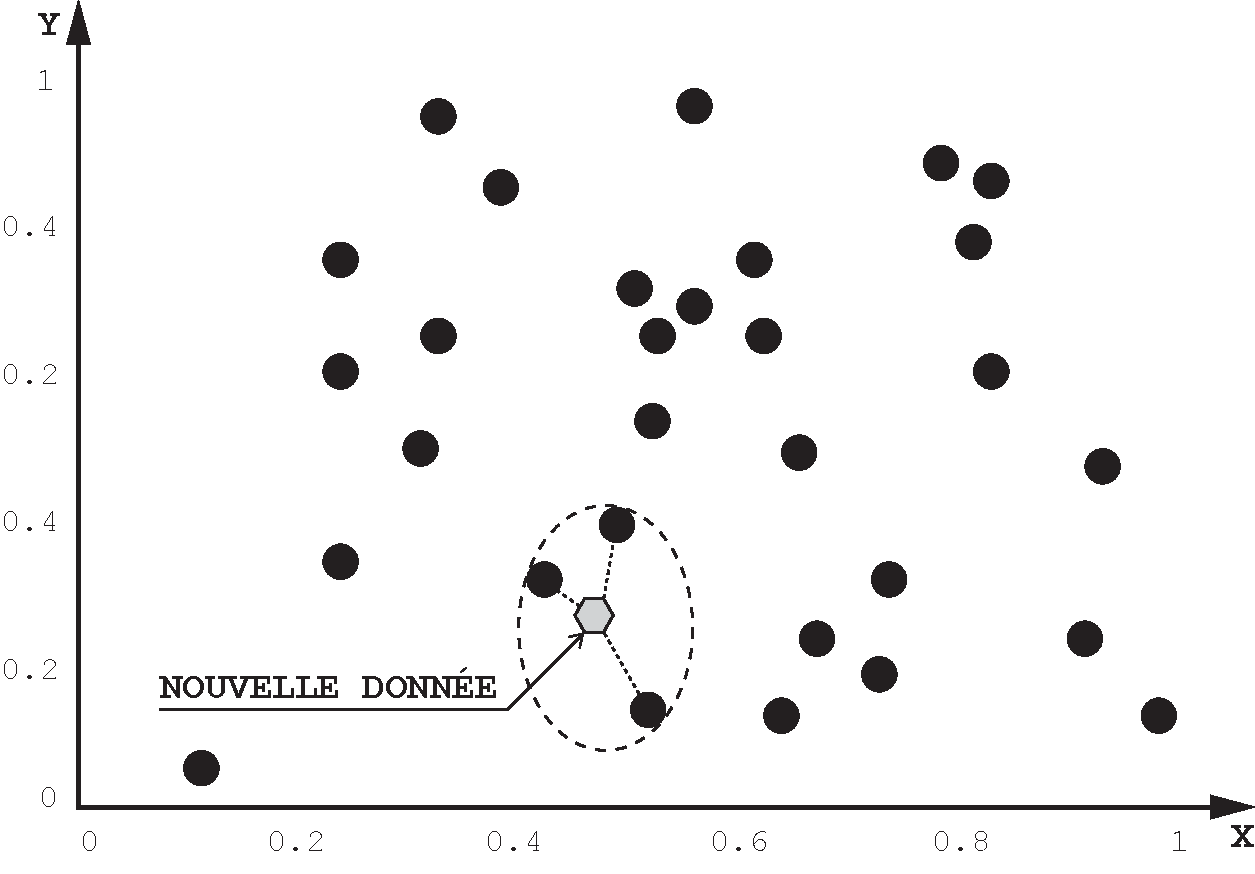
\includegraphics[width=10cm]{algo_knn.pdf}
        \caption{Exemple de l'algoritme des $k$ plus proches voisins où $k=3$.}
	\label{fig:algo_knn}
\end{figure}

\section{Expérimentations}

\subsection{Mise en \oe{}uvre}

\begin{figure}[H]
	\centering
	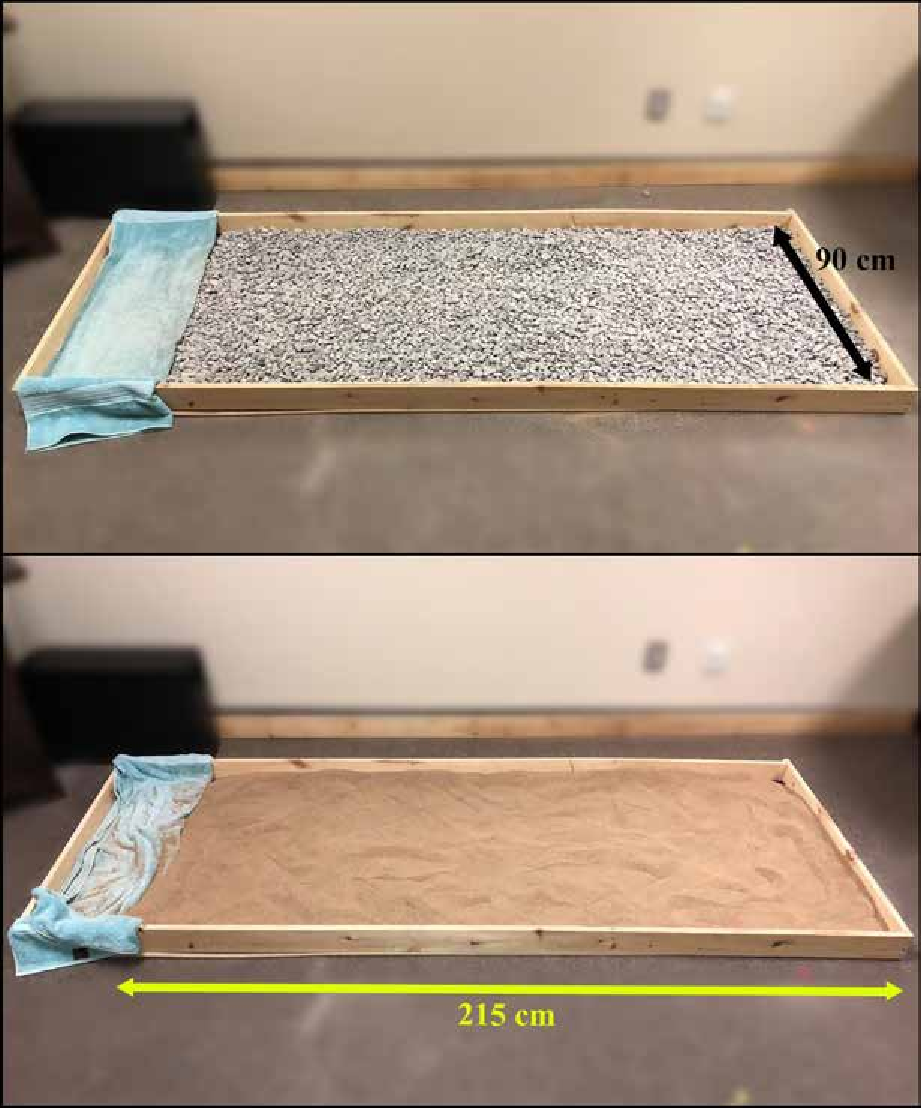
\includegraphics[width=.8\linewidth]{box.pdf}
        \caption{Boîte utilisée lors des expérimentations remplie de gravier et de sable.}
	\label{fig:box}
\end{figure}

\begin{figure}[H]
	\centering
	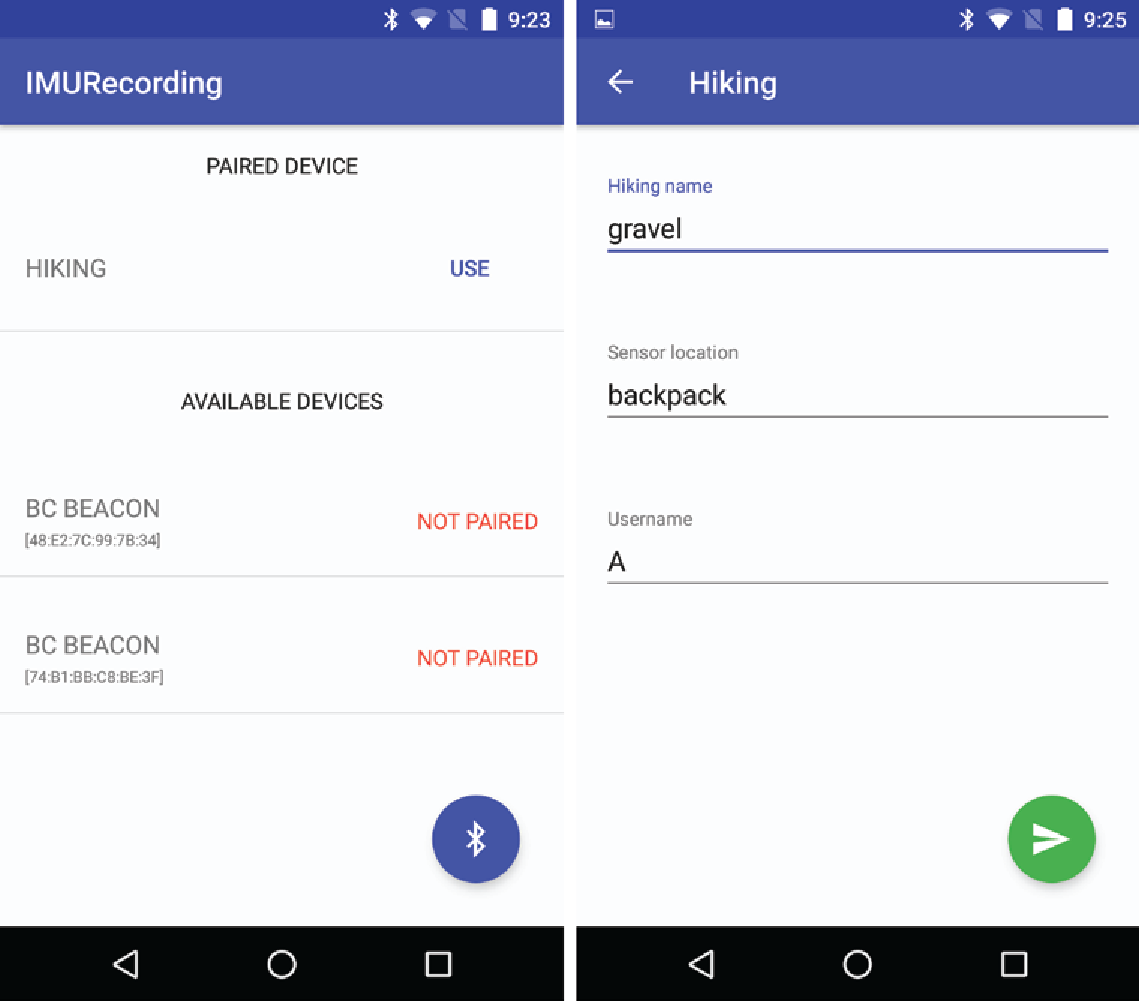
\includegraphics[width=.8\linewidth]{application.pdf}
        \caption{Captures d'écran de l'application \textit{Android} qui permet de piloter et d'étiquetter les données enregistrées.}
	\label{fig:application}
\end{figure}

%To compare our wearable device with a mobile phone, a dedicated application was developed to record the values of the embedded 9-axis IMU. Such a record was achieved on a \textit{Huawei Nexus 6P} running \textit{Android} 8.0 and a stable frequency of 60 Hz was also set for this setup. As for our wearable device, the three Euler angles were calculated and finally, all data were stored in the flash memory of the phone.

% To compare the acquisition of inertial data generated by our wearable device with inertial data that came from a mobile phone, an Android application was specially developed. This application was in charge of recording all the values produced by the 9-axis IMU embedded in the phone (\textit{i.e.} \textit{Huawei Nexus 6P} running the 8.0 version of \textit{Android}) at the same stable frequency as the one offered by our wearable device (\textit{i.e.} 60 Hz). For each data coming from the IMU, the three Euler angles are calculated and this set of twelve values is temporarily stored in a buffer. Its content is finally formatted with configuration values and written on the flash memory of the mobile phone at every second, in the same format as for the wearable device.

\subsection{Procédure}

\begin{figure}[H]
    \centering
	\subfloat[De gauche à droite, positionnement du \textit{wearable device} dans les poches de droite (1) et de gauche (2) ainsi qu'à l'intérieur d'un sac à dos ordinaire de 20L.]{
		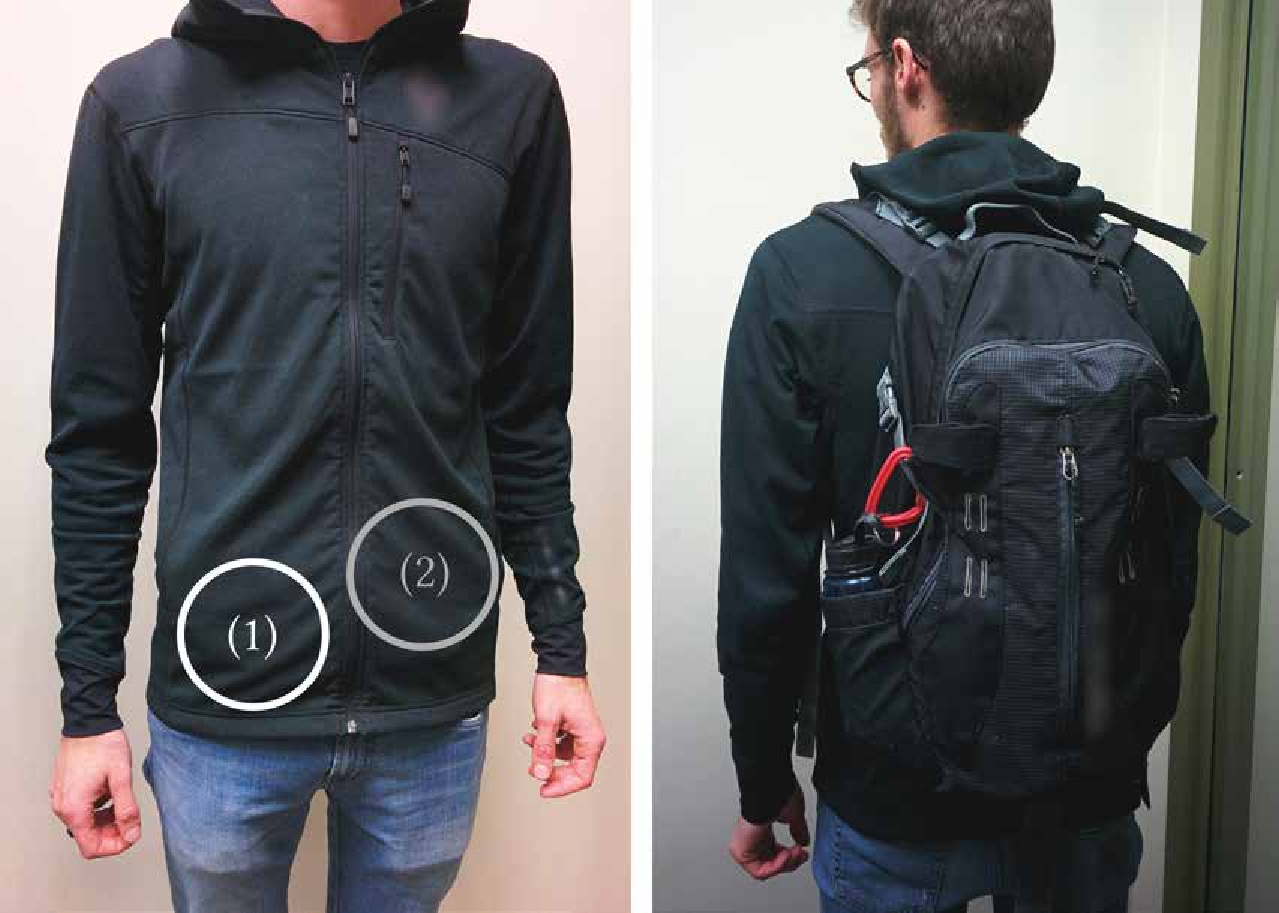
\includegraphics[width=.7\linewidth]{positions_a.pdf}
		\label{fig:positions_a}
    }
    \\[30pt]
	\subfloat[Positionnement du \textit{wearable device} à l'intérieur d'un sac bandoulière porté sur les épaules de droite et de gauche.]{
		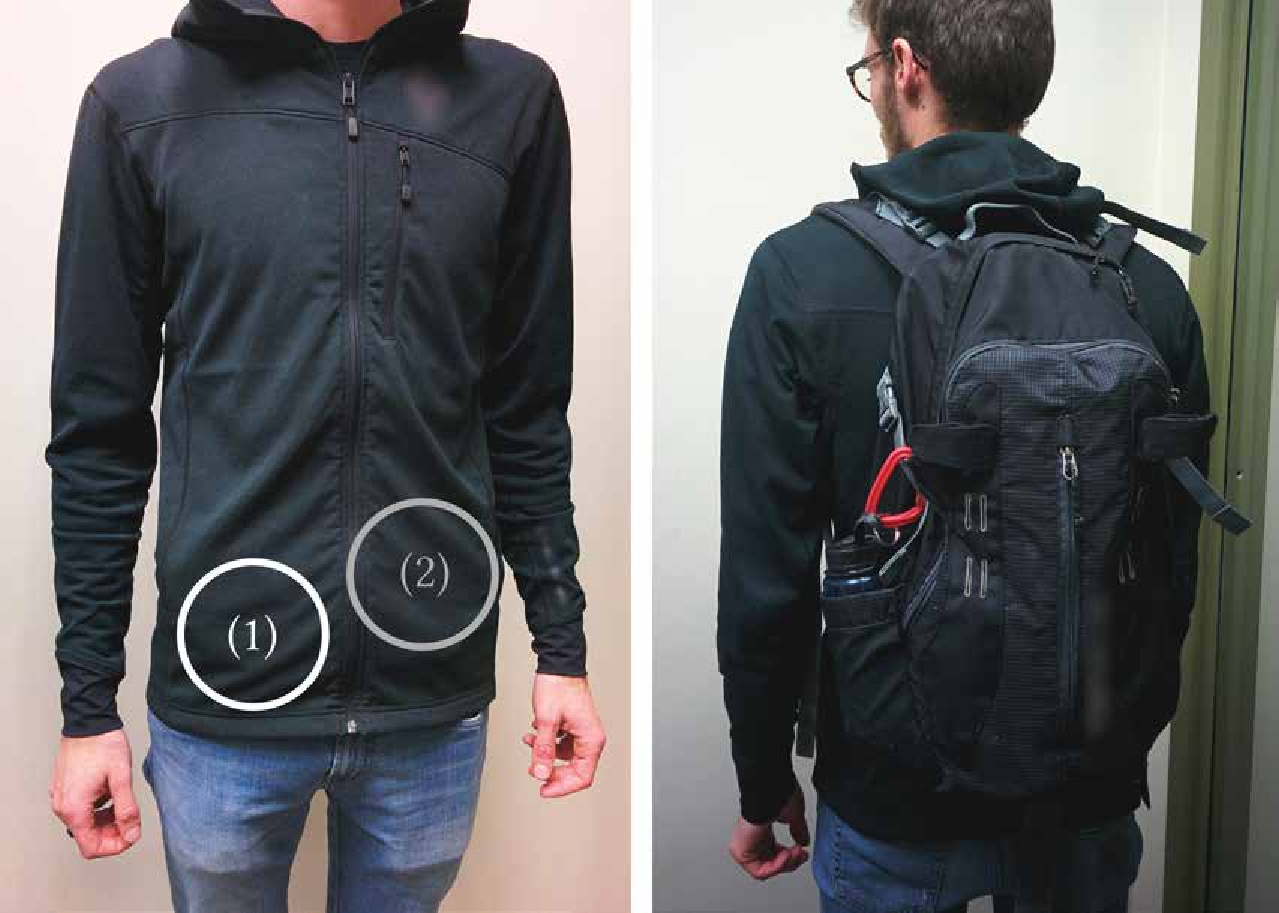
\includegraphics[width=.7\linewidth]{positions_b.pdf}
		\label{fig:positions_b}
    }
    \caption{Illustration des cinq emplacements où le \textit{wearable device} est positionné pendant l'expérimentation.}
    \label{fig:positions}
\end{figure}

\section{Résultats et discussion}

\subsection{Ensembles de données}

\subsection{Résultats obtenus}

\subsection{Discussion des résultats obtenus}

\section{Conclusion}